\documentclass[11pt]{article}

\usepackage[margin=1in]{geometry}
\usepackage[backend=bibtex, style=authortitle, citestyle=authoryear-icomp, url=false]{biblatex}
\usepackage{amsmath, amssymb, amsthm, mathrsfs}
\usepackage{caption, graphicx}
\usepackage{secdot, sectsty}
\usepackage{bbm}
\usepackage{fancyhdr}
\usepackage{listings}
\usepackage{color}
\usepackage{enumitem}
\usepackage{booktabs}
\usepackage{hyperref}
\usepackage{inconsolata}

\newcommand{\inv}[1]{#1^{-1}}
\newcommand{\iid}{\text{i.i.d.}}
\newcommand{\bmat}[1]{\begin{bmatrix} #1 \end{bmatrix}}
\newcommand{\asconv}{\xrightarrow{a.s.}}
\newcommand{\pconv}{\xrightarrow{p}}
\newcommand{\dconv}{\xrightarrow{d}}
\newcommand{\msconv}{\xrightarrow{m.s.}}
\newcommand{\liminfty}{\lim_{n \to \infty}}
\newcommand*\diff{\mathop{}\!\mathrm{d}}
\newcommand{\lhood}{\mathcal{L}}
\renewcommand{\vec}[1]{\mathbf{#1}}

\newtheorem*{proposition}{Proposition}
\newtheorem*{claim}{Claim}

\let\oldforall\forall
\let\forall\undefined
\DeclareMathOperator{\forall}{\oldforall}
\DeclareMathOperator{\ev}{E}
\DeclareMathOperator{\var}{Var}
\DeclareMathOperator*{\argmax}{arg\,max}
\DeclareMathOperator*{\argmin}{arg\,min}

\lstset{
  basicstyle=\footnotesize\ttfamily,
  columns=fixed,
  fontadjust=true,
  basewidth=0.5em
}

\allsectionsfont{\rmfamily}
\sectionfont{\normalsize}
\subsectionfont{\normalfont\normalsize\selectfont\itshape}
\subsubsectionfont{\normalfont\normalsize\selectfont\itshape}

\sectiondot{subsection}

\renewcommand\thesection{\Roman{section}}
\renewcommand\thesubsection{\thesection.\Alph{subsection}}
\renewcommand\thesubsubsection{\thesubsection.\arabic{subsubsection}}

\linespread{1}
\pagestyle{fancy}
\rhead{Econ 210C Homework 2}
\lhead{Justin Abraham}

\begin{document}

\section{Investment and the Housing Market}

    Consider the following model of the housing market $I = \psi(P)$ where $\psi' > 0$ is demand for investment, $R(H)$ where $R' < 0$ is the rental cost of the house as a function of housing stock, $r + \delta = P^{-1}(R + \dot P)$ equates the user cost and the rental rate, and the law of motion for housing is $\dot H = I - \delta H$.

    \begin{enumerate}

        \item It is reasonable to expect that $\psi' > 0$ and $R' < 0$ so that housing follows the law of demand in the rental and asset markets. The condition $r + \delta = P^{-1}(R + \dot P)$ equates the value of real estate with its opportunity cost. Lastly, the model is closed with 4 endogenous variables and 4 equations.

        \item We can reduce the system to two dynamic equations.

            $$ \begin{cases}
            \dot H & = \psi(P) - \delta H \\
            \dot P & = P(r + \delta) - R(H)
            \end{cases} $$

        \item Imposing the steady state yields $H = \delta^{-1} \psi(P)$ and $P = R(H) (r + \delta)^{-1}$. Without knowing $\psi(P)$ or $R(H)$ we at least know that $\frac{dH}{dP} > 0$ on the $\dot H = 0$ locus and $\frac{dH}{dP} < 0$ on the $\dot P = 0$ locus. $H$ converges toward the $\dot H = 0$ locus when out of steady state while $P$ diverges out.

        \item A higher $r$ is associated with lower prices and housing stock in the steady state. This occurs through a rise in $R$ and a decline in $I$.

        \item An unexpected, permanent increase in $r$ will shift the $\dot P = 0$ locus towards the origin. Prices will immediately jump down to the new saddle path but at the same level of housing. Housing stock will decrease gradually to the new steady state. Investment will follow the transition of prices and rental rates will follow the transition of the housing stock.

        \item An unexpected, temporary increase in $r$ will shift the $\dot P = 0$ locus towards the origin as in the permanent case. Prices will immediately decrease after the announcement but to a lesser extent than with a permanent shock. Once the new $r$ takes effect, the dynamics will decumulate capital and increment $P$. Once the transitory shock subsides, $P, H$ will be on the stable path and housing will gradually increase to the original steady state.

        \item When a permanent rise in $r$ is known ahead of time, prices will decrease in anticipation of the shock. As the shock occurs housing stock will adjust to a lower steady state following the stable arm but the change will not be as large as for unexpected shocks due to anticipatory behavior.

        \item Suppose consumers have static expectations about the price of housing so $\ev(\dot P) = 0$. Intuitively, this means that signals about future price changes will not affect current behavior. In this model, prices will immediately jump down to the new saddle path in response to the shock. Housing stock will decrease gradually to the new steady state. Investment will follow the transition of prices and rental rates will follow the transition of the housing stock.

        \item We can use this to model backward-looking, rather than rational, expectations of price changes. When agents extrapolate future prices from histories, they may not correctly anticipate shifts until they already materialize (as in the housing crisis).

    \end{enumerate}

\section{Discount Factor Shocks}

    Consider the model developed in class and allow the discount factor $\beta$ to exogenously vary over time. This variation captures the idea that impatience to consume can fluctuate and it can be interpreted as a demand shock. This modification changes the consumer's Euler equation and rental rate determination.

        $$ \frac{C_{t+1}}{C_t} = \beta_t (1 + R_{t+1}) = \beta_t (\alpha Y_{t+1} K_t^{-1} + (1-\delta)) $$

    A linear approximation is given by log-linearizing.

        $$ \ln C_{t+1} - \ln C_t = \ln \beta_t + \ln (\alpha Y_{t+1} K_t^{-1} + (1-\delta)) $$
        $$ \ev \check C_{t+1} - \check C_t = \check \beta_t + \frac{\alpha \bar Y \bar K}{\alpha \bar Y \bar K + (1-\delta)} (\ev \check Y_{t+1} - \check K_t) $$

    $\check \beta_t$ only enters the costate dynamic equation, which becomes

        $$ \Delta \check \lambda_{t+1} = - \check \beta_t - \frac{\alpha \bar Y \bar K}{\alpha \bar Y \bar K + (1-\delta)} \bigg [ \bigg ( 1 + \frac{1-\alpha}{\alpha+\eta^{-1}} \bigg ) \check Z_{t+1} + (1-\alpha) \bigg ( \frac{\alpha}{\alpha + \eta^{-1}} - 1 \bigg ) \check K_t + \frac{1-\alpha}{\alpha+\eta^{-1}} \check \lambda_{t+1} \bigg ] $$

    A positive discounting shock ($\beta < \beta'$) must be accompanied by a decrease in the marginal product of capital to maintain steady state consumption and investment. In the case of a permanent shock, $\check \lambda$ immediately jumps up to the new stable arm while $\check K$ transitions to a higher steady state following this path. Households have a greater motive to save in the short term but the marginal product of capital will decrease in the long term.

    In the case of a transitory shock, $\check \lambda$ will likewise jump up but fall short of the new stable arm. $\check K$ will gradually increase and $\check \lambda$ will decrease during the transition phase during the shock. The path will inflect towards the original stable arm and reach it after the shock subsides. Tables \ref{tab:permbetashock} and \ref{tab:tempbetashock} summarize the effect on the endogenous variables from a permanent and transitory shock, respectively.

    \begin{table}[h] \centering
    \caption{Comparative statics of a permanent demand shock}
    \label{tab:permbetashock}
    \begin{tabular}{p{2.5cm}p{2.5cm}p{2.5cm}p{2.5cm}}
    \hline
     & Impact & Transition & Steady State \tabularnewline
    \hline
    Consumption & -- & + & + \tabularnewline
    Output & + & ? & + \tabularnewline
    Investment & + & -- & + \tabularnewline
    Employment & + & ? & ? \tabularnewline
    Wages & -- & + & + \tabularnewline
    Interest Rate & + & -- & -- \tabularnewline
    \hline
    \end{tabular}
    \end{table}

    \begin{table}[h] \centering
    \caption{Comparative statics of a transitory demand shock}
    \label{tab:tempbetashock}
    \begin{tabular}{p{2.2cm}p{2.2cm}p{2.2cm}p{2.2cm}p{2.2cm}p{2.2cm}}
    \hline
     & Impact & Transition & Inflection & Transition & Steady State \tabularnewline
    \hline
    Consumption & -- & + & 0 & -- & 0 \tabularnewline
    Output & + & ? & 0 & ? & 0 \tabularnewline
    Investment & + & -- & 0 & + & 0 \tabularnewline
    Employment & + & ? & 0 & -- & 0 \tabularnewline
    Wages & -- & + & 0 & -- & 0 \tabularnewline
    Interest Rate & + & -- & 0 & + & 0 \tabularnewline
    \hline
    \end{tabular}
    \end{table}

\section{Fake News}

    Returning to the classical RBC model as before, consider a positive productivity shock announced at $t_0$ and expected to occur in the future $t_1$ but is not realized. Suppose that the shock is such that $\bar \lambda < \bar \lambda_0$ and $\bar K > \bar K_0$. Initially, variables will transition as if facing an anticipated productivity shock. $\check \lambda$ will jump down just shy of the new stable arm so that $\check \lambda, \check K$ would have moved onto the new stable arm once the permanent shock occurs. Instead, $\check K$ decrements and $\check \lambda$ moves up until cross the $\Delta \check \lambda = 0$ locus where consumption will make a drastic jump so that the economy once again reaches the stable arm. It follows this towards the steady state. Table \ref{tab:permnewsshock} summarizes the effect on the endogenous variables from a permanent shock.

    % Does this mean we cannot recover the old steady state?
    % At $t_1$, $\check \lambda$ jumps back to the original stable path and capital gradually decumulates to the original steady state.
    % possible to fudge the saddle path so that lambda jumps up instead

    \begin{table}[h] \centering
    \caption{Comparative statics of a permanent news shock}
    \label{tab:permnewsshock}
    \begin{tabular}{p{2.5cm}p{2.5cm}p{2.5cm}p{2.5cm}p{2.5cm}}
    \hline
     & Impact & Inflection & Transition & Steady State \tabularnewline
    \hline
    Consumption & + & -- & + & 0 \tabularnewline
    Output & + & -- & ? & 0 \tabularnewline
    Investment & + & -- & -- & 0 \tabularnewline
    Employment & -- & ? & ? & 0 \tabularnewline
    Wages & + & -- & + & 0 \tabularnewline
    Interest Rate & + & + & -- & 0 \tabularnewline
    \hline
    \end{tabular}
    \end{table}

\section{Labor Supply}

    Suppose an individual with a $T$ period horizon wants to consume a constant level of consumption $C$ per period. She earns $w$ per hour, she must decide how many hours $N$ to work per period. The path of the wage rate $w_t$ is known at $t=0$. The rate of time preference and of interest are zero. The individual's problem is $\min_{\{N_t\}} \sum_{t=0}^T \ln(1+N_t)$ subject to $CT = \sum_{t=0}^T w_t N_t$ and $N_t \geq 0$.

    \begin{enumerate}

        \item The Euler equation for intertemporal labor supply is $w_t (1 + N_t) = w_s (1 + N_s) \forall s, t \leq T$.

        \item The individual works to equalize the ratio of marginal utility and marginal product of labor across periods. In an environment with a constant wage, no discounting, and perfect foresight, the individual will work the same amount each period.

        \item This theory produces several testable implications. Under the proposed model, labor supply should have a positive relationship with contemporaneous wage changes and a negative relationship with announced, future changes.

        \item Households will work more in the periods after an unexpected, permanent increase in wage in order to equalize the ratio of marginal utility and marginal product (a substitution effect).

        \item If a delayed but expected, permanent wage increase were to occur, household will work less today and compensate by working more after the wage hike.

        \item Labor supply elasticity is positive with respect to contemporaneous wages ($\varepsilon_L = 1$) but negative with respect to future wages due to intertemporal substitution.

    \end{enumerate}

\section{Impulse Responses by Simulation}

    Assume $\check G = 0$ and $\check L = 0$.

    \begin{enumerate}

        \item Table \ref{tab:volatilities} compares simulated volatilities with those calculated in Stock and Watson (S\&W). Consumption exhibits the least volatility while investment the most as expected. These are lower that estimated by S\&W overall.

        \item Figure \ref{fig:imp1_impulse} plots the impulse response of the linearized model. Since capital is a predetermined stock, it increases continuously in response to the shock and returns to the steady state gradually. Consumption and investment, as choice variables, jump immediately after the shock with investment being more senitive due to consumption smoothing. Wages and output respond immediately as functions of $\check C, \check I$ but are slowed down by $\check K$.

        \item Suppose that $\rho = 1$ so that the technology shock persists indefinitely. As expected, consumption, investment, output, capital, and wages maintain higher steady state levels. The jump in consumption is more severe in response to unanticipated, permanent shocks to be able to reach the new stable arm.

        \item Suppose $\alpha = \frac{2}{3}$. The factor share is a scaling term on the marginal product of capital and the linearized production technology in the case of inelastic labor. A higher $\alpha$ means that output and wages wil be more senitive to the dynamics of capital. With a transitory shock we observe as much compared to the baseline model. With a permanent shock, capital, output, wages, and investment resolve to a higher steady state. Table \ref{tab:volatilities} compares simulated volatilities with those calculated in S\&W and the baseline model. Again, consumption exhibits the least volatility while investment the most as expected. These are still lower that estimated by S\&W overall. Compared to baseline, output and investment are much more volatile.

        \item So far we've used first moments from data to calibrate parameters. To match observed volatilities we must calibrate using higher moments. Note that we cannot use the same set of moments to calibrate \emph{and} evaluate the model due to overfitting.

    \end{enumerate}

    \begin{figure}[h]
        \centering
        \caption{Impulse response for a unit productivity shock}
        \label{fig:imp1_impulse}
        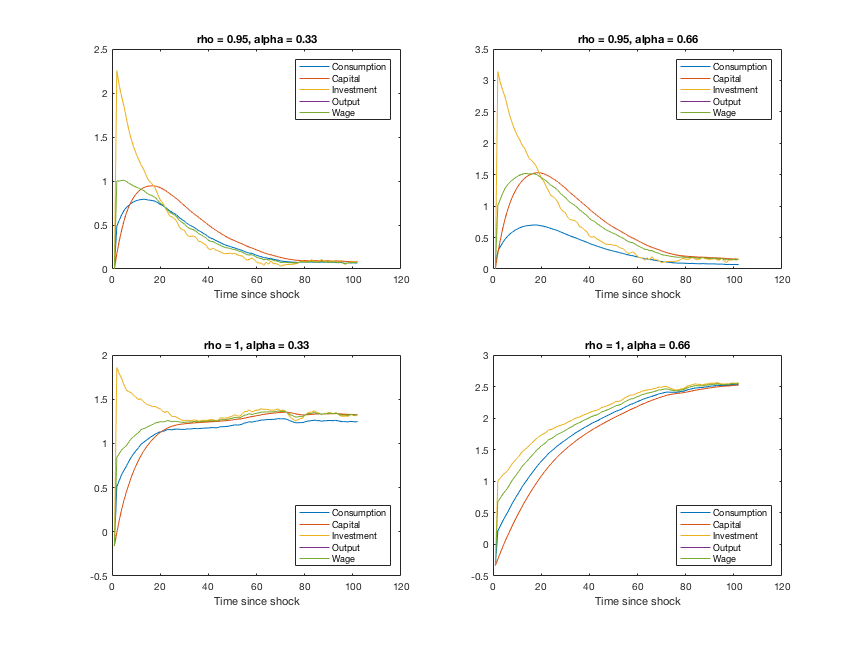
\includegraphics[width=\textwidth]{imp1_impulse.png}
    \end{figure}

    \begin{table}[h] \centering
    \caption{Simulated volatilities of aggregate variables (std. dev.)}
    \label{tab:volatilities}
    \begin{tabular}{p{2.5cm}p{2.5cm}p{2.5cm}p{2.5cm}}
    \hline
     & $\alpha = \frac{1}{3}$ & $\alpha = \frac{2}{3}$ & S\&W \tabularnewline
    \hline
    Output & 0.0695 & 0.1209 & 1.66 \tabularnewline
    Consumption & 0.0583 & 0.0562 & 1.26 \tabularnewline
    Investment & 0.1035 & 0.1582 & 4.97 \tabularnewline
    \hline
    \end{tabular}
    \end{table}

\section{Impulse Responses with Dynare}

    \begin{enumerate}
        \item Figure \ref{fig:imp2_impulse} plots the impulse response functions for several endogenous variables (in log units).
        \item Investment responds more severely to the productivity shock than consumption, capital, and output as in the simulation. Overall, the log-linearization seems to have produced comparable results to the untransformed model.
    \end{enumerate}

    \begin{figure}[h]
        \centering
        \caption{Impulse response for a unit productivity shock}
        \label{fig:imp2_impulse}
        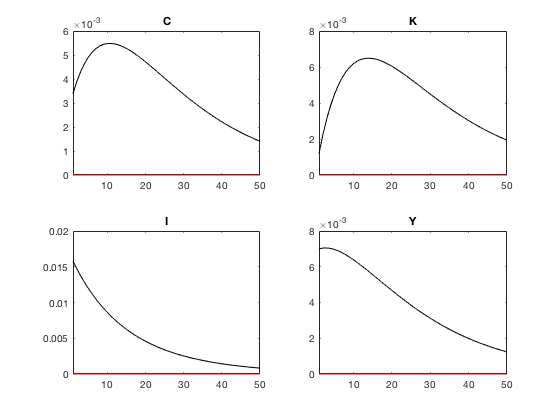
\includegraphics[width=\textwidth]{imp2_impulse.png}
    \end{figure}

\clearpage

\appendix

\newpage

\section{RBC Simulation}

    \lstinputlisting{Abraham_210C_sim.m}

\newpage

\section{Solving RBC with Dynare}

    \lstinputlisting{Abraham_210C_HW2.mod}

\end{document}
